% ##################################################################################################################
\chapter{Tel Aviv}
\label{ch:telaviv}
\hfill \textbf{Author:} Christoph Dobler

\editdone{This text has undergone the professional edit. Please no grammatical changes anymore! They are most-probably wrong.}

% ##################################################################################################################
The initial Tel Aviv \gls{matsim} scenario \citep[][]{BekhorEtAl_TRB_2011} was recently extended by adding destination choice to the \gls{matsim} iterations \citep[][]{DoblerEtAl_TechRep_IVT_2014}.

The modeled area was divided into 1\,219\,\gls{taz} (Figure~\ref{fig:TAZ}); geometry was provided as a \gls{esri} shape file \citep{ESRI-ShapeFile_manual_1998}. Zonal attributes contained information on the population living in the zone, as well as types of activities that can be performed.

The population was created using population generator outcomes from the Tel Aviv activity-based model, containing socio-demographic attributes and daily schedules with up to six activities. This kept computational effort manageable; a 10\,\% population sample was simulated. Additional data was provided for external trips; for each of the three types (car, truck, commercial), \gls{od} matrices for three different time periods were available.

Network input data was taken from the \gls{emme2} model \citep[see][]{EMME_Webpage_2015}, also used by the Assignment Unit of the existing Tel Aviv Model. Conversion process details can be found in \citet{GaoWEtAl_TRR_2010}. Turning restrictions were handled by adapting the network structure, resulting in a network containing 9\,474\,nodes and 18\,570\,links (Figure~\ref{fig:network}). Some major road capacities were obviously too low (\eg noticeably lower than traffic counts indicated) and were corrected manually.

The Tel Aviv scenario contained road pricing for two arterial highways; count data for validation was available for three arterial roads.
%\karen{ Why do we have 3 here instead of the word three? I notice it has a \, after it.. is this a special notation?  thanks...}.
%
\createfigure%
{Tel Aviv scenario}%
{Tel Aviv scenario}%
{\label{fig:telavivscenario}}%
{%
  \createsubfigure%
  {\protect\gls{taz}}%
  {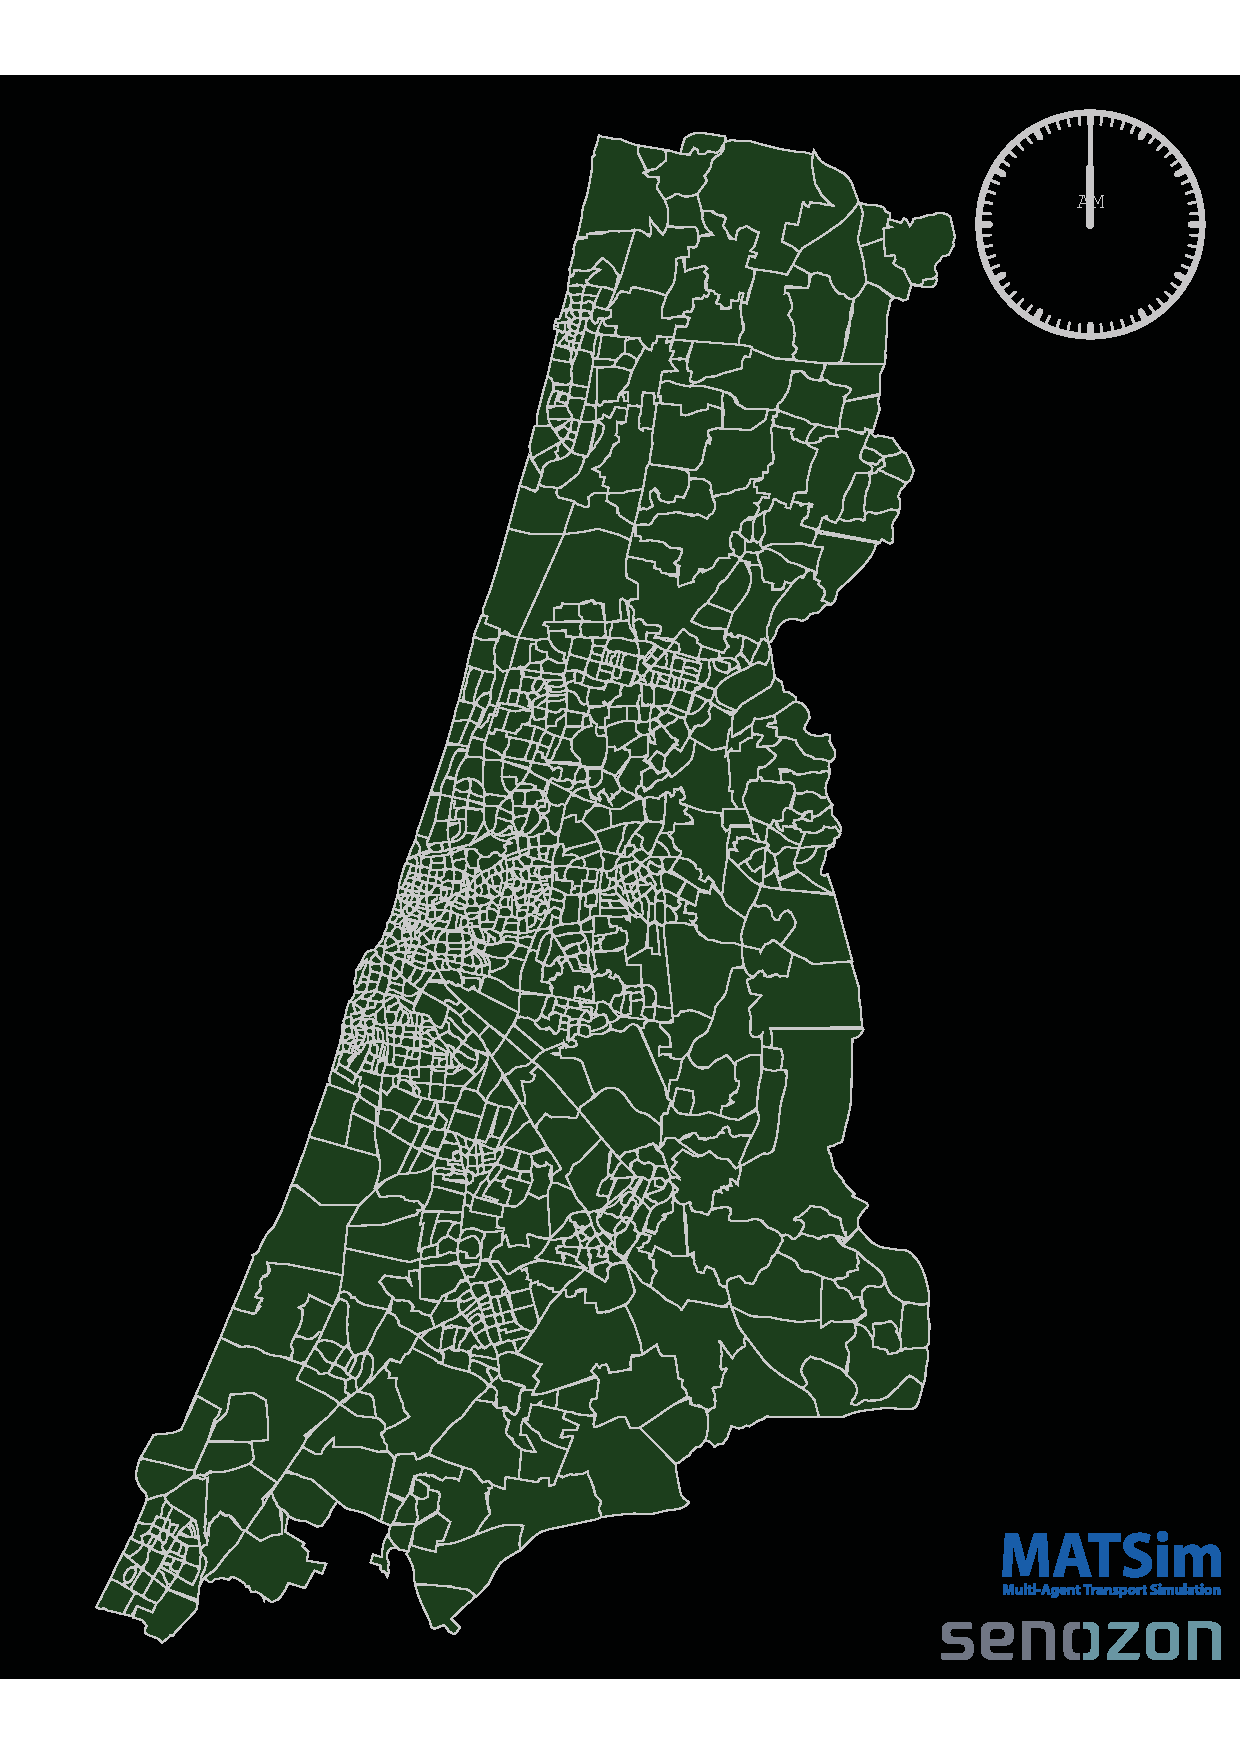
\includegraphics[width=0.49\textwidth,angle=0]{scenarios/figures/TelAviv_TAZ}}%
  {\label{fig:TAZ}}%
  {}%
  \createsubfigure%
  {Network}%
	{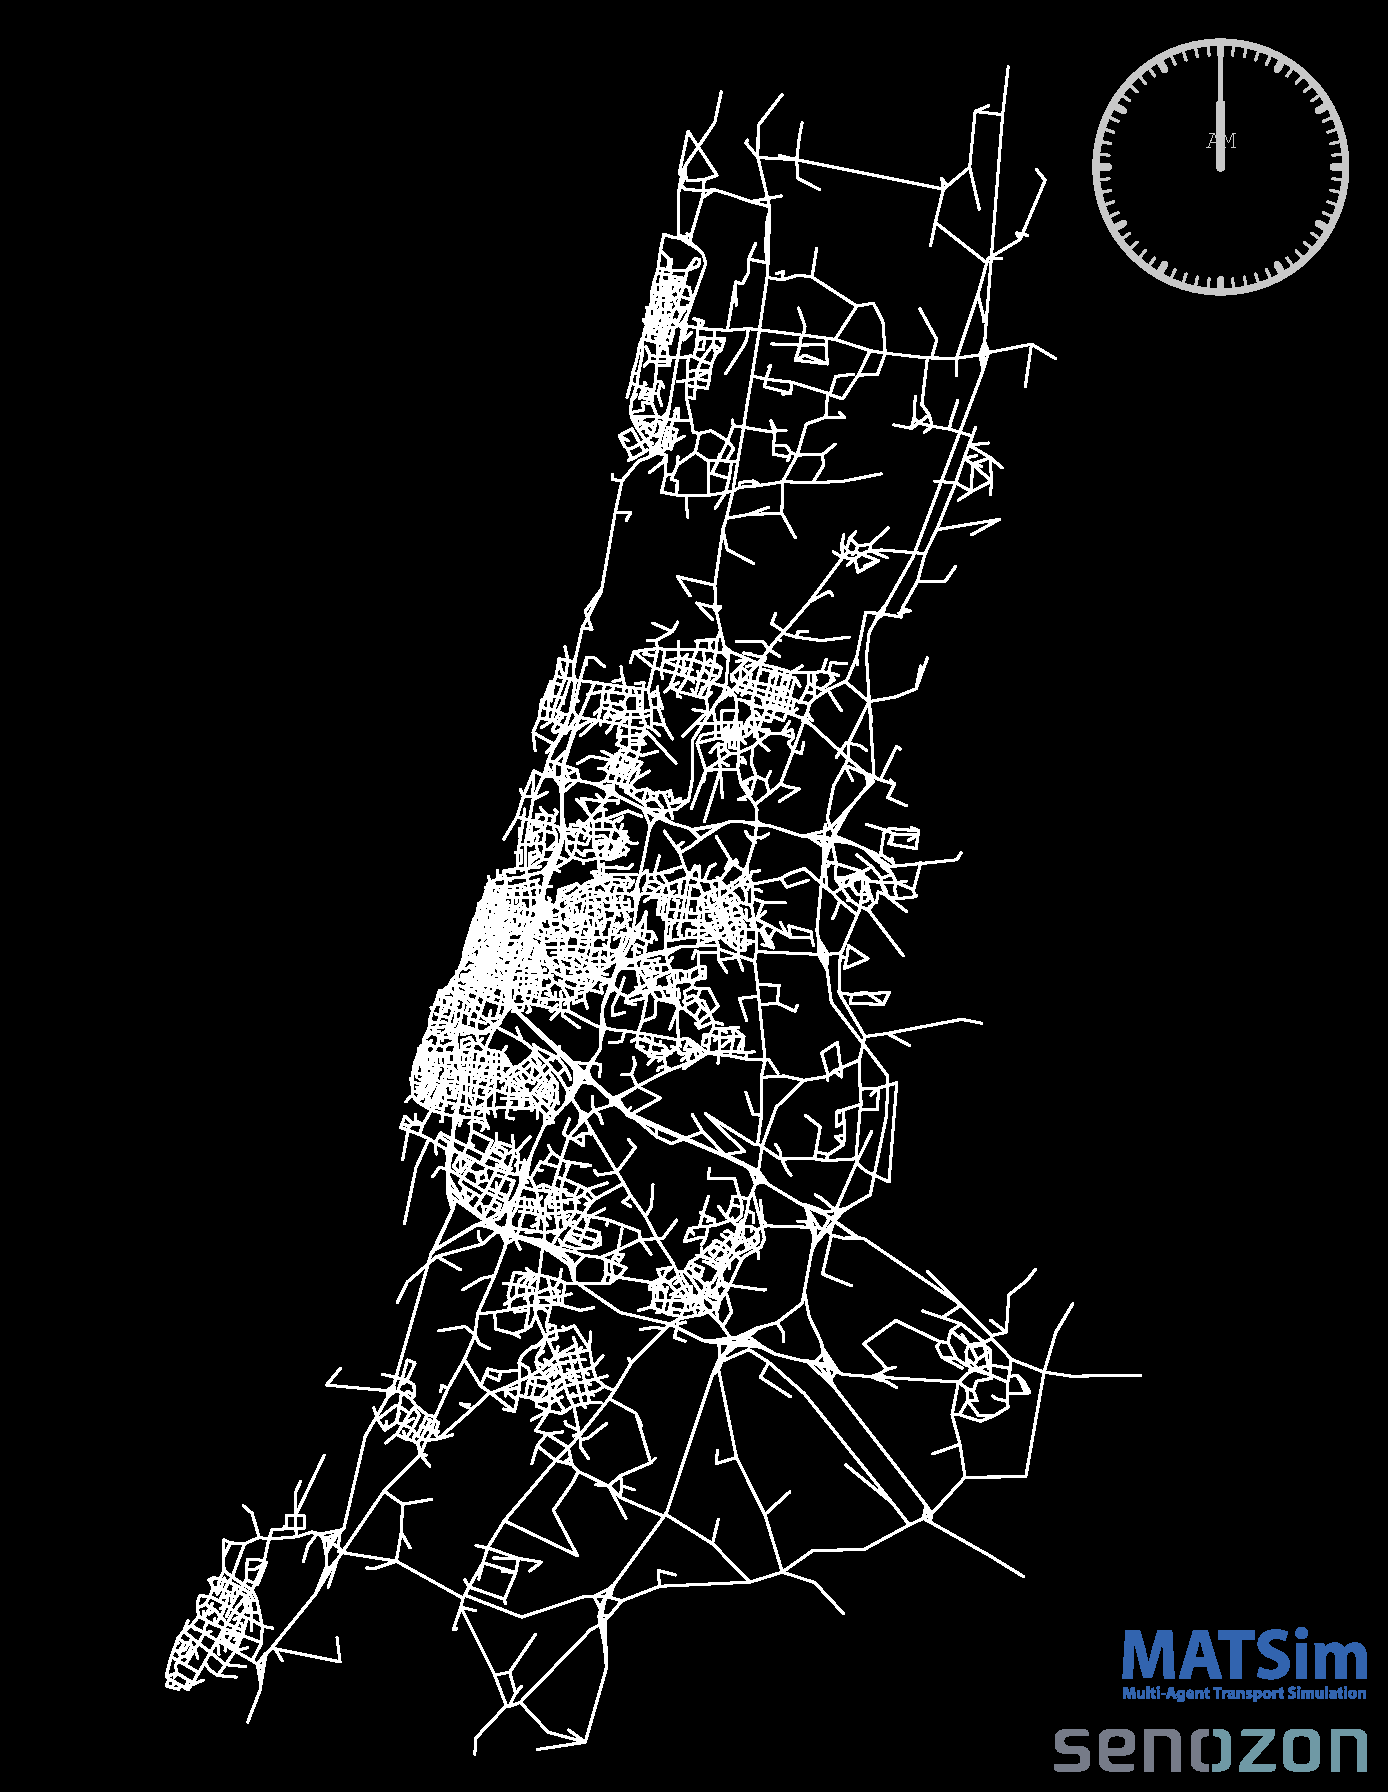
\includegraphics[width=0.49\textwidth,angle=0]{scenarios/figures/TelAviv_RoadNetwork}}%
  {\label{fig:network}}%
  {}%
}%
{}

% ##################################################################################################################
